\documentclass[12pt]{article}
\usepackage[russian]{babel}
\usepackage[utf8x]{inputenc}
\usepackage{amssymb}
\usepackage{amsmath}
\usepackage{graphicx}
\usepackage{geometry}
\usepackage[colorinlistoftodos]{todonotes}
\usepackage{listings}
\usepackage[section]{placeins}
\begin{document}

\title{1. Гармонический анализ непериодических сигналов}
\author{Андрей Валиков}
\date{}
\maketitle
																																																								\section{Математическая модель сигнала}
Исходный сигнал:
\begin{gather*}
x(t) = 
\begin{cases}
  Ae^{-t/\tau} \text{ if $0\leq t\leq T_c$}\\
  0 \text{ else}    
\end{cases}
\end{gather*}

\noindent Константы имеют следующие значения:
\[A = 2\]
\[\tau = 0.5\]
\[T_c = 0.7\]

\begin{lstlisting}
A, tau = 2, .5
def _func(arg):

  return A * np.exp(-arg / tau) if 0 <= arg.all() < t[-1] else 0

N  = 300
t  =  np.linspace(0, .7, N)

func = _func(t)

ax1 = plt.subplot(221)
ax1.plot(t, func, 'r')
ax1.set_title('Original')
\end{lstlisting}

\begin{figure}[htp]
\centering
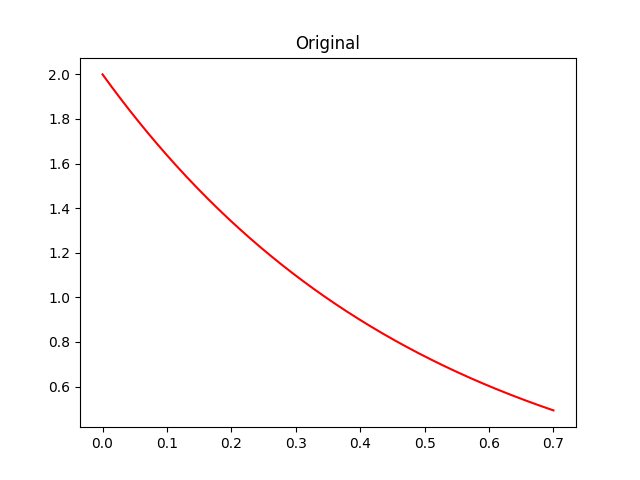
\includegraphics[scale=1.00]{original.png}
\caption{}
\label{}
\end{figure}

\section{Амплитудная и фазовая спектральные характеристики полученные с помощью прямого преобразования Фурье.}
Используется тригонометрическая форма преобразования Фурье:

\[\hat{f}(\omega) = \int_{-\infty}^{\infty}x(t)\cos(\omega t)dt -
 i\int_{-\infty}^{\infty}x(t)\sin(\omega t)dt\]
 
\noindent Модуль полученной спектральной характеристики будет составлять амплитудную характеристику сигнала:
\[A(\omega) = |\hat{f}|\]
А аргумент фазовую:
\[\Phi(\omega) = \arg \hat{f}\]

\begin{lstlisting}
fou = []
om  = np.linspace(0, 2000, N)
for i in range(N):
  re = np.trapz(func * np.cos(t * om[i]), x=t)
  im = np.trapz(func * np.sin(t * om[i]), x=t)
  fou.append(re - im * 1j)

ax2 = plt.subplot(223)
ax2.plot(om, np.abs(fou))
ax2.set_title('Amplitudes')

ax3 = plt.subplot(224)
ax3.plot(om, np.angle(fou))
ax3.set_title('Frequencies')
\end{lstlisting}

\begin{figure}[!htb]
\centering
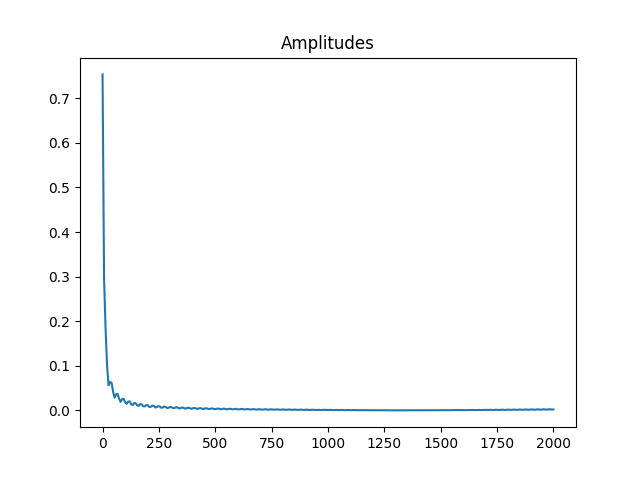
\includegraphics[scale=1.00]{amplitudes.png}
\caption{}
\label{}
\end{figure}

\begin{figure}[!htb]
\centering
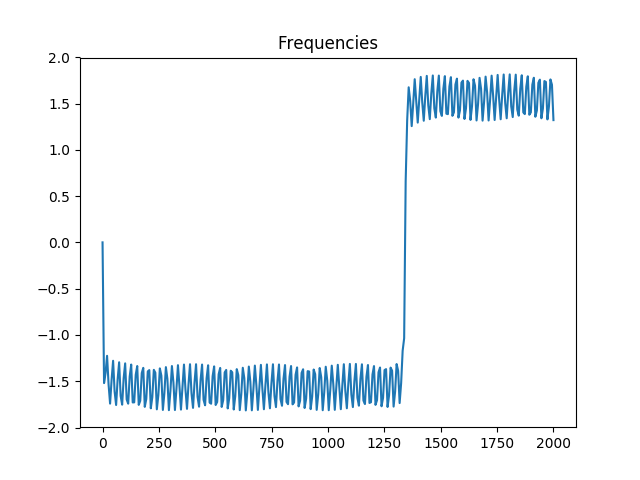
\includegraphics[scale=1.00]{frequencies.png}
\caption{}
\label{}
\end{figure}

\section{Восстановление функции с помощью обратного преобразования Фурье}

\[f(t) = \frac{1}{\pi} \int_{0}^{\infty}(\operatorname{Re}(\hat{f})\cos(\omega t) - \operatorname{Im}(\hat{f})\sin(\omega t))d\omega \]

\begin{lstlisting}
rst  = []
for i in range(N):
  a = np.trapz(np.real(fou) * np.cos(om * t[i]), x = om)
  b = np.trapz(np.imag(fou) * np.sin(om * t[i]), x = om)
  rst.append((a - b) / np.pi)

ax4 = plt.subplot(222)
ax4.plot(t, rst, 'g')
ax4.set_title('Restored')
\end{lstlisting}

\begin{figure}[htp]
\centering
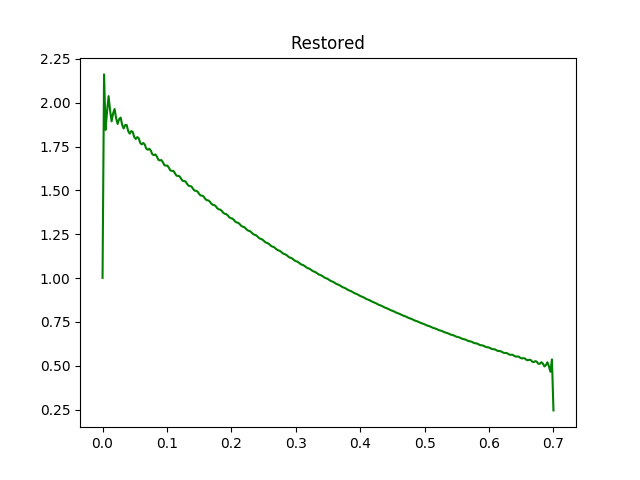
\includegraphics[scale=1.00]{restored.png}
\caption{}
\label{}
\end{figure}

\section{Вывод}
Имеется исходный сигнал, экспонента на интервале [0, Tc], нулевое значение на остальных аргументах.\\
С помощью прямого преобразования Фурье получается Фурье образ, комплексный ряд.\\
По известным формулам получен амплитудный спектр (модуль). И фазовую (аргумент)\\
Обратное преобразование Фурье позволяет восстановить исходную сигнал.


\end{document}